
A ROOT-based system was developed to display integrated quantities from the CLAS trigger system in the form of 1D and 2D histograms. The system is made by three different applications: a histogram sender running on each VTP, a histogram receiver running on a DAQ server, and a user-configurable GUI client.
Each histogram sender application defines a set of 1D and 2D histograms to report trigger data specific to the CLAS12 subsytem handled by the VTP it is running on. Histograms are refreshed at a fixed rate and streamed to the DAQ server in the form of JavaScript Object Notation (JSON) messages, exploiting the previously described ActiveMQ infrastructure. Each message contains: the histogram name, the number of bins, and a data array with the number of counts in each bin.
The message receiver application is responsible for decoding these messages, and of creating ROOT histograms from them. Finally, the client application displays ROOT histograms to the user through a customizable GUI. The GUI is composed of a programmable number of independent frames, with different histograms in each of them. Typically, each frame contains histograms related to the same CLAS12 subsystem. The GUI structure is specified through a configuration file passed as a command-line option when running the client. Communication between the message receiver/ROOT histogram produced application and the user client is handled through the ROOT TSocket mechanism.
Fig.~\ref{fig:plot_andrea} shows a GUI reporting histograms from the Forward Tagger system \cite{ft-ref}: two 2D histograms showing the distribution of electromagnetic clusters seed hits in the Forward Tagger Calorimeter, and two 1D histograms showing the electromagnetic cluster energy distribution. The right (left) column report histograms for electromagnetic clusters  with (without) a matching hit in the Forward Tagger Hodoscope.

\begin{figure*}[t]
	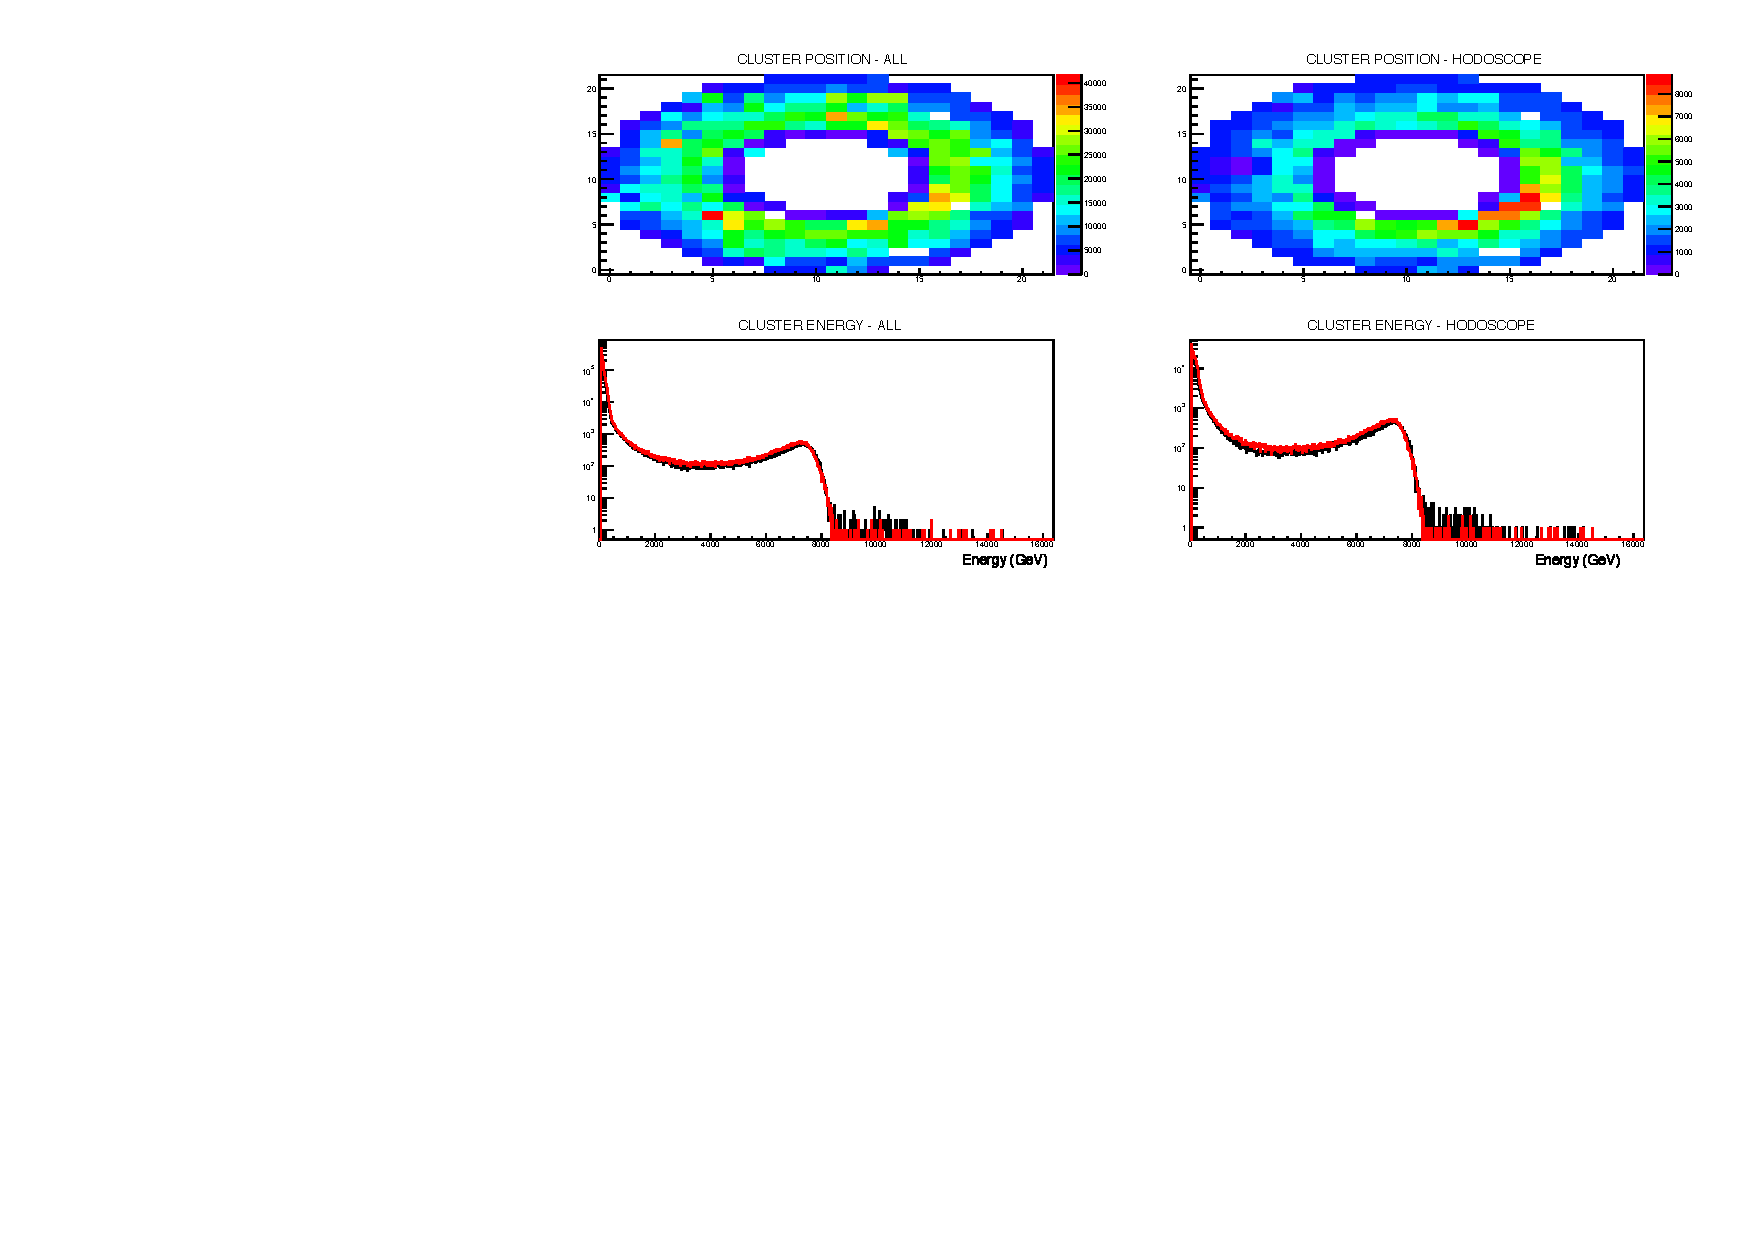
\includegraphics[width=\textwidth]{img/plotAndrea.pdf}
	\caption{Example of a ROOT-based GUI to monitor trigger data, for the specific case of the Forward Tagger detector. Top histograms report the distribution of electromagnetic clusters seed hit positions, while the bottom histograms report the electromagnetic clusters energy distribution. Right (left) column report histograms for electromagnetic clusters  with (without) a matching hit in the Forward Tagger Hodoscope.}
	\label{fig:plot_andrea}
\end{figure*}
